\documentclass[11pt]{article}
\usepackage[margin=2cm]{geometry}
\usepackage{FabPackages4}
\bibliography{bibliography}

% Custom commands
\captionsetup{labelfont=bf, font=bf}
\newcommand{\note}[1]{\vspace{10mm}\caption*{\small #1}}


\title{\textbf{Stata-Latex Integration} \\ -- A simple example -- }
\author{Fabian Gunzinger}
\date{\today}



\begin{document}

\maketitle


% ===========================================================================
\section{Introduction}
% ===========================================================================

Some text here. Let's cite \citet{acemoglu2001colonial} and \citet{kahneman1979prospect} to look a bit more credible.



% ===========================================================================
\section{Data}
% ===========================================================================

Where you explain what data you use and document how you cleaned it and constructed variables.



% ===========================================================================
\section{Results}
% ===========================================================================

Table \ref{tab:results} shows something you can explain here...

Figure \ref{fig:bars} shows something. 


\begin{table}[h]\centering \def\sym#1{\ifmmode^{#1}\else\(^{#1}\)\fi} \caption{Average treatment effect} \label{tab:results} \maxsizebox*{\textwidth}{\textheight}{ \begin{threeparttable} \begin{tabular}{lcc} \toprule
                    &\multicolumn{1}{c}{(1)}         &\multicolumn{1}{c}{(2)}         \\
\hline
Intervention        &       7.376\sym{*}  &       8.401\sym{*}  \\
                    &      (2.09)         &      (2.41)         \\
[1em]
Registered voters   &                     &      0.0577\sym{***}\\
                    &                     &     (15.08)         \\
[1em]
Constant            &       392.6\sym{***}&       337.6\sym{***}\\
                    &     (42.87)         &     (34.76)         \\
[1em]
Town fixed-effects  &         Yes         &         Yes         \\
\hline
Mean turnout untreated&       461.3         &       461.3         \\
Observations        &        6970         &        6948         \\
\bottomrule \end{tabular} \begin{tablenotes}[flushleft] \footnotesize \item The columns present results from regressing total turnout on an intervention dummy and different sets of control variables. The coefficient on the intervention variable is an estimate of the average treatment effect. Values in parenteses are t statistics. * denotes significance at 10 pct., ** at 5 pct., and *** at 1 pct. level. \end{tablenotes} \end{threeparttable} } \end{table}



\begin{figure}[h]\centering
\caption{Catchy title comes here
\label{fig:bars}}
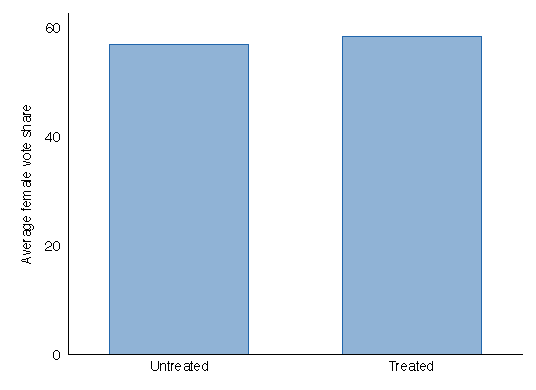
\includegraphics[width=.49\textwidth]{../analysis/output/fig-bars.pdf}
\captionsetup{belowskip=-30pt, font=normalfont, width=.5\textwidth}
\note{\footnotesize Illuminating footnote explaining what's going on in the figure comes here (though the figure really shouldn't need that much explanation).}
\end{figure}




% ===========================================================================
\section{Appendix}
% ===========================================================================

The histograms in Figure \ref{fig:histograms} show some more things.


\begin{figure}[H]\centering
\caption{Distributions of registered voters and turnout
\label{fig:histograms}}
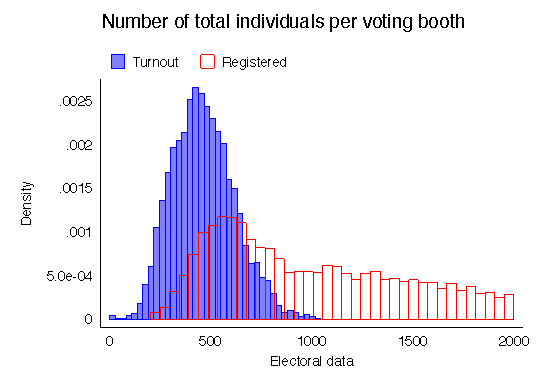
\includegraphics[width=.32\textwidth]{../analysis/output/fig-hist-total.pdf}
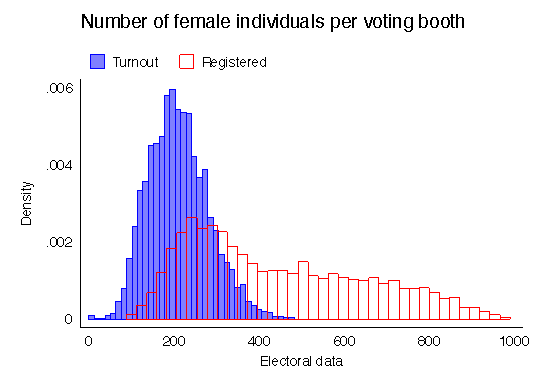
\includegraphics[width=.32\textwidth]{../analysis/output/fig-hist-female.pdf}
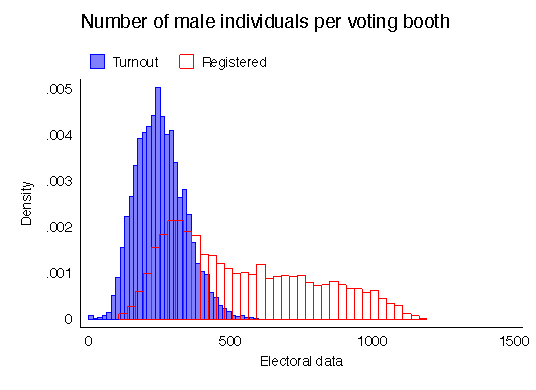
\includegraphics[width=.32\textwidth]{../analysis/output/fig-hist-male.pdf}
\captionsetup{belowskip=-10pt, font=normalfont, width=.94\textwidth}
\end{figure}


\newpage
\printbibliography

\end{document}
